\documentclass[a4paper, 12pt]{article}%тип документа

%Русский язык
\usepackage[T2A]{fontenc} %кодировка
\usepackage[utf8]{inputenc} %кодировка исходного кода
\usepackage[english,russian]{babel} %локализация и переносы

%отступы 
\usepackage[left=2cm,right=2cm,top=2cm,bottom=3cm,bindingoffset=0cm]{geometry}

%Вставка картинок
\usepackage{graphicx}
\graphicspath{}
\DeclareGraphicsExtensions{.pdf,.png,.jpg, .jpeg}

%Таблицы
\usepackage[table,xcdraw]{xcolor}
\usepackage{booktabs}

%Графики
\usepackage{pgfplots}
\pgfplotsset{compat=1.9}

%Математика
\usepackage{amsmath, amsfonts, amssymb, amsthm, mathtools}

%Заголовок
\author{Подлесный Артём \\ группа 827}
\title{Работа 1.2.5 \\ Исследование прецессии уравновешенного гироскопа}

\begin{document}
\maketitle
\section{Цель работы}
Исследовать вынужденную прецессию гироскопа. Установить зависимость скорости вынужденной прецессии от величины момента сил, действующих на ось гироскопа. Определить скорость вращения ротора гироскопа и сравнить ее со скоростью, рассчитанной по скорости прецессии.
\section{Оборудование}
Гироскоп в кардановом подвесе, секундомер, набор грузов, отдельный ротор гироскопа, цилиндр известной массы, крутильный маятник, штангенциркуль, линейка.
\section{Отчёт о работе}
\subsection{Общая теория}
Уравнения движения твердого тела можно записать в виде:
\begin{equation}
\dfrac{d\vec{P}}{dt}=\vec{F},
\end{equation}
\begin{equation}
\dfrac{d\vec{L}}{dt}=\vec{M}.
\end{equation}
Здесь (1) выражает закон движения центра масс тела, а (2) -- уравнение моментов. Если сила $\vec{F}$ не зависит от угловой скорости, а момент сил -- от поступательного движения, то уравнения (1) и (2) можно рассматривать независимо друг от друга. В данной работе  мы рассматриваем вращение твердого тела относительно неподвижной точки. Момент импульса твердого тела в XYZ равен 
\begin{equation}
\vec{L}=\vec{i}I_{\text{x}}\omega_{\text{x}}+\vec{j}I_{\text{y}}\omega_{\text{y}}+\vec{k}I_{\text{z}}\omega_{\text{z}},
\end{equation}
где $I_{\text{x}}$, $I_{\text{y}}$, $I_{\text{z}}$ -- главные моменты инерции, $\omega_{\text{x}}$, $\omega_{\text{y}}$, $\omega_{\text{z}}$, -- компоненты вектора угловой скорости $\vec{\omega}$. Быстро вращающееся тело, для которого, например,
\[I_{\text{x}}\omega_{\text{x}}\gg I_{\text{y}}\omega_{\text{y}}, I_{\text{z}}\omega_{\text{z}},\]
Принято называть гироскопом. Гироскоп называют уравновешенным, если его центр масс неподвижен. \\
Так как приращение момента импульса по (2) определяется, как
\begin{equation}
\Delta\vec{L}=\int\vec{M}dt,
\end{equation}
то если момент сил действует короткий промежуток времени, изменение момента импульса очень мало, по сравнению с ним, с этим связана устойчивость, которую приобретает движение гироскопов, после приведение их в быстрое вращение. \\
Рассмотрим для примера маховик, вращающийся вокруг оси $z$.
\\
\\
\\ \\ \\ \\ \\ \\ \\ \\ \\ \\ \\ \\ \\
\\
\\
\\
Пусть ось вращения повернулась в плоскости $xy$ по направлению к оси $x$ на бесконечно-малый угол $d\varphi$. Такой поворот означает добавочное вращение вокруг оси $y$, где $\Omega$ --- угловая скорость такого вращения. Будем предполагать, что 
\begin{equation}
L_{\Omega} \ll L_{\omega_0}.
\end{equation}
Таким образом: 
\begin{equation}
\mid d\vec{L}\mid=Ld\varphi=L\Omega dt.
\end{equation}
Но это изменение направлено по оси $x$, поэтому вектор $d\vec{L}$ можно представить, как
\[d\vec{L}=\left[ \vec{\Omega};\vec{L}\right] dt,\]
т.е. в силу (2) имеем
\begin{equation}
\vec{M}=\left[ \vec{\Omega};\vec{L}\right].
\end{equation}
Формула (7) справедлива, когда справедлива формула (5). Она позволяет определить момент сил, который надо приложить к маховику для того, чтобы вызвать вращение маховика с угловой скоростью $\vec{\Omega}$. Видно, что для поворота оси вращающегося маховика к оси $x$ необходимо приложить силы, направленные не вдоль оси $x$, а вдоль оси $y$, так, чтобы их момент был направлен вдоль оси $x$. \\
Под действием момента внешних сил ось гироскопа медленно вращается вокруг оси $y$ с угловой скоростью $\Omega$. Такое движение называют регулярной прецессией. В частности, создающей момент внешней силой может быть сила тяжести, если центр масс гироскопа не совпадает с точкой подвеса. Для гироскопа массой $m_{\text{г}}$, ось которого наклонена на угол $\alpha$ от вертикали, скорость прецессии равна:
\begin{equation}
\Omega=\dfrac{M}{I_z\omega_0\sin\alpha}=\dfrac{m_{\text{г}}gl_{\text{ц}}\sin\alpha}{I_z\omega_0\sin\alpha}=\dfrac{m_{\text{г}}gl_{\text{ц}}}{I_z\omega_0},
\end{equation}
где $l_{\text{ц}}$ -- расстояние от точки подвеса до ц.м. гироскопа, то есть от угла $\alpha$ скорость прецессии не зависит.\\
Для изучения уравновешенного гироскопа, к его оси подвешивают дополнительне грузы, в этом случае 
\begin{equation}
\Omega=\dfrac{mgl}{I_z\omega_0},
\end{equation}
где $m$ -- масса груза, а $l$ -- расстояние от центра карданова подвеса, до точки крепления груза на оси гироскопа.

Уравновешенный гироскоп, закрепленный в кольцах карданова подвеса:
\\
\\
\\ \\ \\ \\ \\ \\ \\ \\ \\ \\ \\ \\ \\
\\ \\ \\ \\ \\ \\ \\ \\ \\ \\ \\ \\ \\
\\ \\ \\ 
\\
Получается, что гироскоп как бы подвешен а центр масс.

Экспериментальная установка для исследования прецессии уравновешенного гироскопа:
\\ \\ \\ \\ \\ \\ \\ \\ \\ \\ \\ \\ \\
\\ \\ \\ \\ \\ \\ \\ \\ \\ \\ \\ \\ \\
Момент силы трения, связанной с ротором гироскопа скомпенсирован действием электромотора. Для осей карданова подвеса компенсации нет, поэтому нужно оценить погешность, связанную с постепенным опусканием оси гироскопа в направлении действия груза. 

В первой части работы исследуется зависимость скорости прецессии гироскопа от момента силы, приложенной к его оси. Эта зависимость позволяет вычислить угловую скорость вращения ротора по формуле (9). Момент инерции ротора относительно оси симметрии $I_0$ измеряется по крутильным колебаниям точной копии ротора, подвешиваемой вдоль оси симметрии на жесткой проволоке. Период крутильных колебаний:
\begin{equation}
T_0=2\pi\sqrt{\dfrac{I_0}{f}},
\end{equation}
где $f$ -- модуль кручения проволоки. Чтобы их исключить, к той же проволоке подвесим цилиндр известного момента инерции $I_{\text{ц}}$, тогда имеем:
\begin{equation}
I_0=I_{\text{ц}}\dfrac{T^2_0}{T^2_{\text{ц}}},
\end{equation}
где $T_{\text{ц}}$ -- период крутильных колебаний цилиндра.

Во второй части работы скорость вращения ротора гироскопа измеряется с помощью фигур Лиссажу, полуаемых на осциллографе с обмотки гироскопа и прокаллиброванного генератора.
\subsection{Экспериментальные данные}
\subsubsection{Момент сил трения}
Соберем экспериментальную установку, и приведем её к виду рис.3. Проверяя устойчивость гироскопа при легком постукивании по ручагу С, можно убедится, что вращение ротора происходит достаточно быстро. Эта устойчивость связана с тем, что при небольшом времени воздействия момента внешних сил, приращение момента импульса гироскопа очень мало, данный факт подробнее объяснен в теории. По реакции гироскопа на нажатие на рычаг С определим, в какую сторону вращается ротор:\\
При нажатии на рычаг гироскоп \\ начал вращаться по направлению \\ против часовой стрелки \\ в горизонтальной плоскости.\\ Из распределения моментов сил\\ на рис.4 можно определить \\ направление вектора угловой скорости \\ вращения ротора. Отсюда видно,\\ что он вращается против часовой\\ стрелки в вертикальной плоскости,\\ представленной на рисунке.\\
Из рис.5 можно видеть, в какой оси возникает трение, которое приводит к тому, что рычаг С начинает медленно опускаться:
\begin{flushright}
Рычаг опускается, когда возникает \\небольшая прецессия, вызванная\\ моментом сил трения, как показано \\на рисунке. Из векторных уравнений\\ можно определить, как направлен\\ момент, а из этого найти точку\\ его приложения (в каждый \\момент времени) $\Rightarrow$ найти ось.\\Из рисунка понятно, что это ось ОО.
\end{flushright}
Трение присутствует и в других осях ротора гироскопа, однако его действие компенсирует электрогенератор. Момент силы трения можно посчитать, используя следующую формулу:
\begin{equation}
M_{\text{тр}}=I_z\omega_0\Omega_{\text{тр}}\sin{\alpha}=I_z\omega_0\Omega_{\text{тр}},
\end{equation}
Т.к. в данном случае угол $\alpha$ примерно равен $90^{\circ}$. Здесь $\omega_0$ -- угловая скорость собственного вращения ротора, которую еще необходимо определить.
\subsubsection{Скорость регулярной прецессии}
Измерение скорости регулярной прецессии проводилось следующим образом: на рычаг С по очереди на определенном расстоянии $l_{\text{ц}}=121$ мм  от центра карданова подвеса надевались грузы различной массы. Для каждого из грузов проводилась серия из 3-5 повторений, в которых секундомнером измерялось время, за которое гироскоп совершит какое-то число оборотов прецессии, из чего вычеслялась скорость прецессии: $\Omega=\frac{n}{\tau}$, где $n$ -- число оборотов за время $\tau$. Сразу были вычислены и погрешности для каждого значения $\Omega$. Результаты эксперимента предаставлены в таблице 1.
\begin{table}[h!]
\center{\begin{tabular}{|l|l|l|l|l|l|ll|}
\hline
$m$, г & $M$, Н*м  & $T$, с & $N$, дел & $n$, об & $\Omega$, $c^{-1}$ & \multicolumn{1}{l|}{$\Omega_{\text{ср}}$, $c^{-1}$}     & $\sigma_{\Omega}$, $c^{-1}$ \\ \hline
268  & 0,31779 & 136  & 1      & 3       & 0,022059                   & \multicolumn{1}{l|}{0,02207} & 0,00024 \\ \cline{1-6}
268  & 0,31779 & 228  & 2      & 5       & 0,02193                    & \multicolumn{1}{l|}{}        &         \\ \cline{1-6}
268  & 0,31779 & 183  & 2      & 4       & 0,021858                   & \multicolumn{1}{l|}{}        &         \\ \cline{1-6}
268  & 0,31779 & 90   & 1      & 2       & 0,022222                   & \multicolumn{1}{l|}{}        &         \\ \cline{1-6}
268  & 0,31779 & 217  & 2      & 4,83    & 0,022258                   & \multicolumn{1}{l|}{}        &         \\ \hline
335  & 0,39724 & 183  & 2      & 5       & 0,027322                   & \multicolumn{1}{l|}{0,02733} & 0,00020 \\ \cline{1-6}
335  & 0,39724 & 220  & 2      & 6       & 0,027273                   & \multicolumn{1}{l|}{}        &         \\ \cline{1-6}
335  & 0,39724 & 146  & 2      & 4       & 0,027397                   & \multicolumn{1}{l|}{}        &         \\ \hline
215  & 0,25495 & 229  & 2      & 4       & 0,017467                   & \multicolumn{1}{l|}{0,01695}                      & 0,00056 \\ \cline{1-6}
215  & 0,25495 & 187  & 2      & 3,25    & 0,01738                    & \multicolumn{1}{l|}{}        &         \\ \cline{1-6}
215  & 0,25495 & 125  & 1      & 2       & 0,016                      & \multicolumn{1}{l|}{}        &         \\ \hline
173  & 0,20514 & 73   & 1      & 1       & 0,013699                   & \multicolumn{1}{l|}{0,01406} & 0,00027 \\ \cline{1-6}
173  & 0,20514 & 78   & 1      & 1,08    & 0,013846                   & \multicolumn{1}{l|}{}        &         \\ \cline{1-6}
173  & 0,20514 & 142  & 1      & 2       & 0,014085                   & \multicolumn{1}{l|}{}        &         \\ \cline{1-6}
173  & 0,20514 & 200  & 2      & 2,92    & 0,0146                     & \multicolumn{1}{l|}{}        &         \\ \hline
141  & 0,16720 & 85   & 1      & 1       & 0,011765                   & \multicolumn{1}{l|}{0,01158} & 0,00014 \\ \cline{1-6}
141  & 0,16720 & 167  & 2      & 1,92    & 0,011497                   & \multicolumn{1}{l|}{}        &         \\ \cline{1-6}
141  & 0,16720 & 87   & 1      & 1       & 0,011494                   & \multicolumn{1}{l|}{}        &         \\ \cline{1-6}
141  & 0,16720 & 173  & 2      & 2       & 0,011561                   & \multicolumn{1}{l|}{}        &         \\ \hline
116  & 0,13755 & 108  & 1      & 1       & 0,009259                   & \multicolumn{1}{l|}{0,0093}  & 0,00009 \\ \cline{1-6}
116  & 0,13755 & 215  & 2      & 2       & 0,009302                   & \multicolumn{1}{l|}{}        &         \\ \cline{1-6}
116  & 0,13755 & 106  & 1      & 1       & 0,009434                   & \multicolumn{1}{l|}{}        &         \\ \hline
93   & 0,11028 & 100  & 1      & 0,75    & 0,0075                     & \multicolumn{1}{l|}{0,00751} & 0,00014 \\ \cline{1-6}
93   & 0,11028 & 164  & 2      & 1,25    & 0,007622                   & \multicolumn{1}{l|}{}        &         \\ \cline{1-6}
93   & 0,11028 & 135  & 1      & 1       & 0,007407                   & \multicolumn{1}{l|}{}        &         \\ \hline
\end{tabular}}
\end{table}

Так же эти результаты представлены в виде графика зависимости $\Omega$ от $M$.

\begin{figure}[h!]
\center{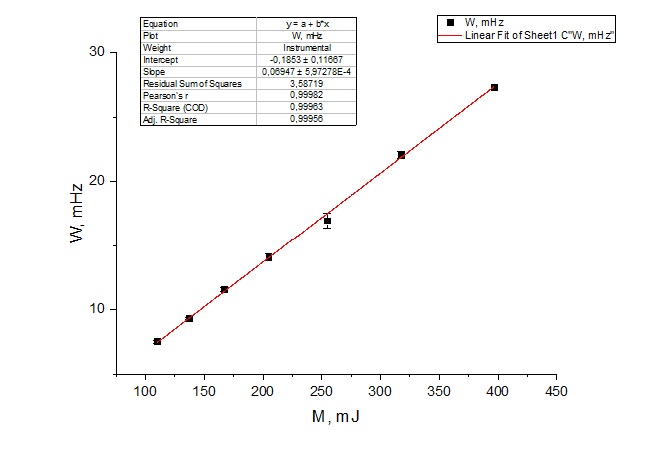
\includegraphics[scale=1.2]{gr1.png}}
\caption{Зависимость $\Omega$ от $M$.}
\end{figure}
Экспериментальные точки аппроксимируются прямой, построеной по методу наименьших квадратов. Теоретическая зависимость для этой прямой такая:
\[\Omega=\dfrac{M}{2\pi I_0\omega_0}.\]
Отсюда, зная коэффициент наклона графика получаем:
\[I_0\omega_0=(2.29\pm0.02) \text{ Дж*с}.\]
Осталось только найти момент инерции ротора $I_0$.
\subsubsection{Момент инерции ротора}
Он вычислялся из формулы (11). К проволоке прикрепляли обычный цилиндр и ротор, и смотрели период крутильных колебаний этих тел. Для каждого из тел была снята серия времён, за которые происходили 10 колебаний. Результаты представлены в таблице:
\begin{table}[h]
\center{\begin{tabular}{|c|c|c|c|c|c|}
\hline
$T_{r10}$, c & $T_{\text{р}}$, c & $\sigma_{T_{\text{р}}}$, c & $T_{c10}$, c & $T_{\text{ц}}$, c & $\sigma_{T_{\text{ц}}}$, c \\ \hline
32,31        &                   &                            & 40,75        &                   &                            \\ \cline{1-1} \cline{4-4}
32,37        &                   &                            & 40,72        &                   &                            \\ \cline{1-1} \cline{4-4}
32,28        & 3,24              & 0,02                       & 40,84        & 4,09              & 0,02                       \\ \cline{1-1} \cline{4-4}
32,5         &                   &                            & 41,05        &                   &                            \\ \cline{1-1} \cline{4-4}
32,38        &                   &                            & 40,97        &                   &                            \\ \hline
\end{tabular}}
\end{table}
Это -- геометрические размеры цилиндра, с помощью которых можно найти  его момент иненрции.
\[m_{\text{ц}}=(1617,9\pm0,1) \text{ г}.\]
\[r_{\text{ц}}=(3,89\pm0,01) \text{ см}.\]
По формуле
\[I_{\text{ц}}=\frac{mr^2}{2},\]
получаем:
\[I_{\text{ц}}=(1.22\pm0.01) \text{ мДж}.\]
Таким образом момент инерции ротора:
\[I_{\text{р}}=(0.77\pm0.02) \text{ мДж}.\]
\subsubsection{Частота вращения ротора}
По известным нам соотношениям легко вычислить $\omega_0$ -- собственную частоту вращения ротора:
\[\omega_0=(473.54\pm16.27) \text{ об/сек}.\]
Зная эту частоту, можно оценить момент сил трения.
\subsubsection{Оценка момента сил трения} 
С помощью формулы (12) оценим момент сил трения, но для начала построим график скорости прецессии из-за трения $\Omega_{\text{тр}}$
от скорости прецессии из-за момента силы тяжести $\Omega_{\text{cр}}$, используя данные таблицы1.

\begin{figure}[h!]
\center{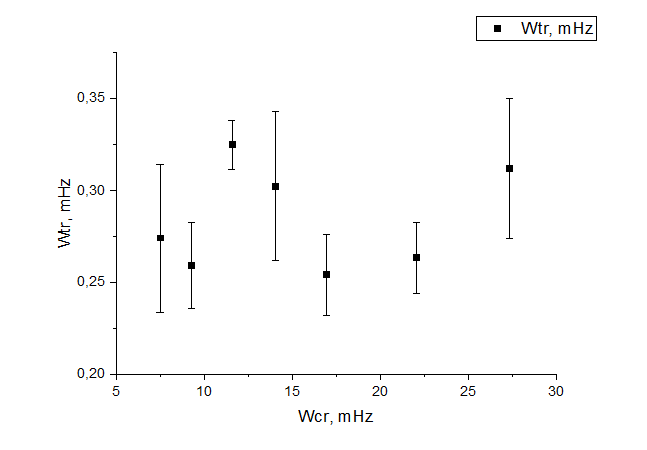
\includegraphics[scale=1.0]{gr2.png}}
\caption{Зависимость $\Omega_{\text{тр}}$ от $\Omega_{\text{cр}}$.}
\end{figure}

По этому рисунку видно, что данные по скорости прецессии носят лишь оценочный характер, потому что они сняты с очень большой неточностью, что связано с утановкой, поэтому имеет смысл лишь оценивать значение момента сил трения и его вклад по сравнению с моментом сил тяжести груза. Как видно из таблицы, он очень мал.

\begin{table}[h]
\center{\begin{tabular}{|l|l|l|l|l|l|l|l|}
\hline
$M_{\text{тр}}$, мДж & 3,777 & 4,48  & 3,644 & 4,341 & 4,663 & 3,72 & 3,933 \\ \hline
$M$, мДж             & 317,8 & 397,2 & 255   & 205   & 167   & 138  & 110   \\ \hline
\%                   & 1,19  & 1,13  & 1,43  & 2,12  & 2,79  & 2,70 & 3,58  \\ \hline
\end{tabular}}
\end{table}

Таким образом, момент сил трения меньше момента сил тяжести груза примерно на 2 порядка и составляет $\approx 10^{-3} \text{ Дж}$.
\subsection{Определение частоты через фигуры Лиссажу}
После того, как установка была приведена в нужное положение, были получены результаты резонансной частоты для включенного генератора:
\[\omega_r=(489\pm 1) \text{ Гц},\] 
и только что выключенного:
\[\omega_r=(464\pm 1) \text{ Гц}.\]
Так как когда генератор включен, он мешает измерению (наводит ЭДС в обмотке выхода, ведущего к осциллографу), то следует считать более достоверным результат, который был получен сразу при выключении генератора, то есть 464 Гц. Он должен совпадать с частотой вращения ротора. Фигура Лиссажу при этом результате:

\begin{figure}[h!]
\center{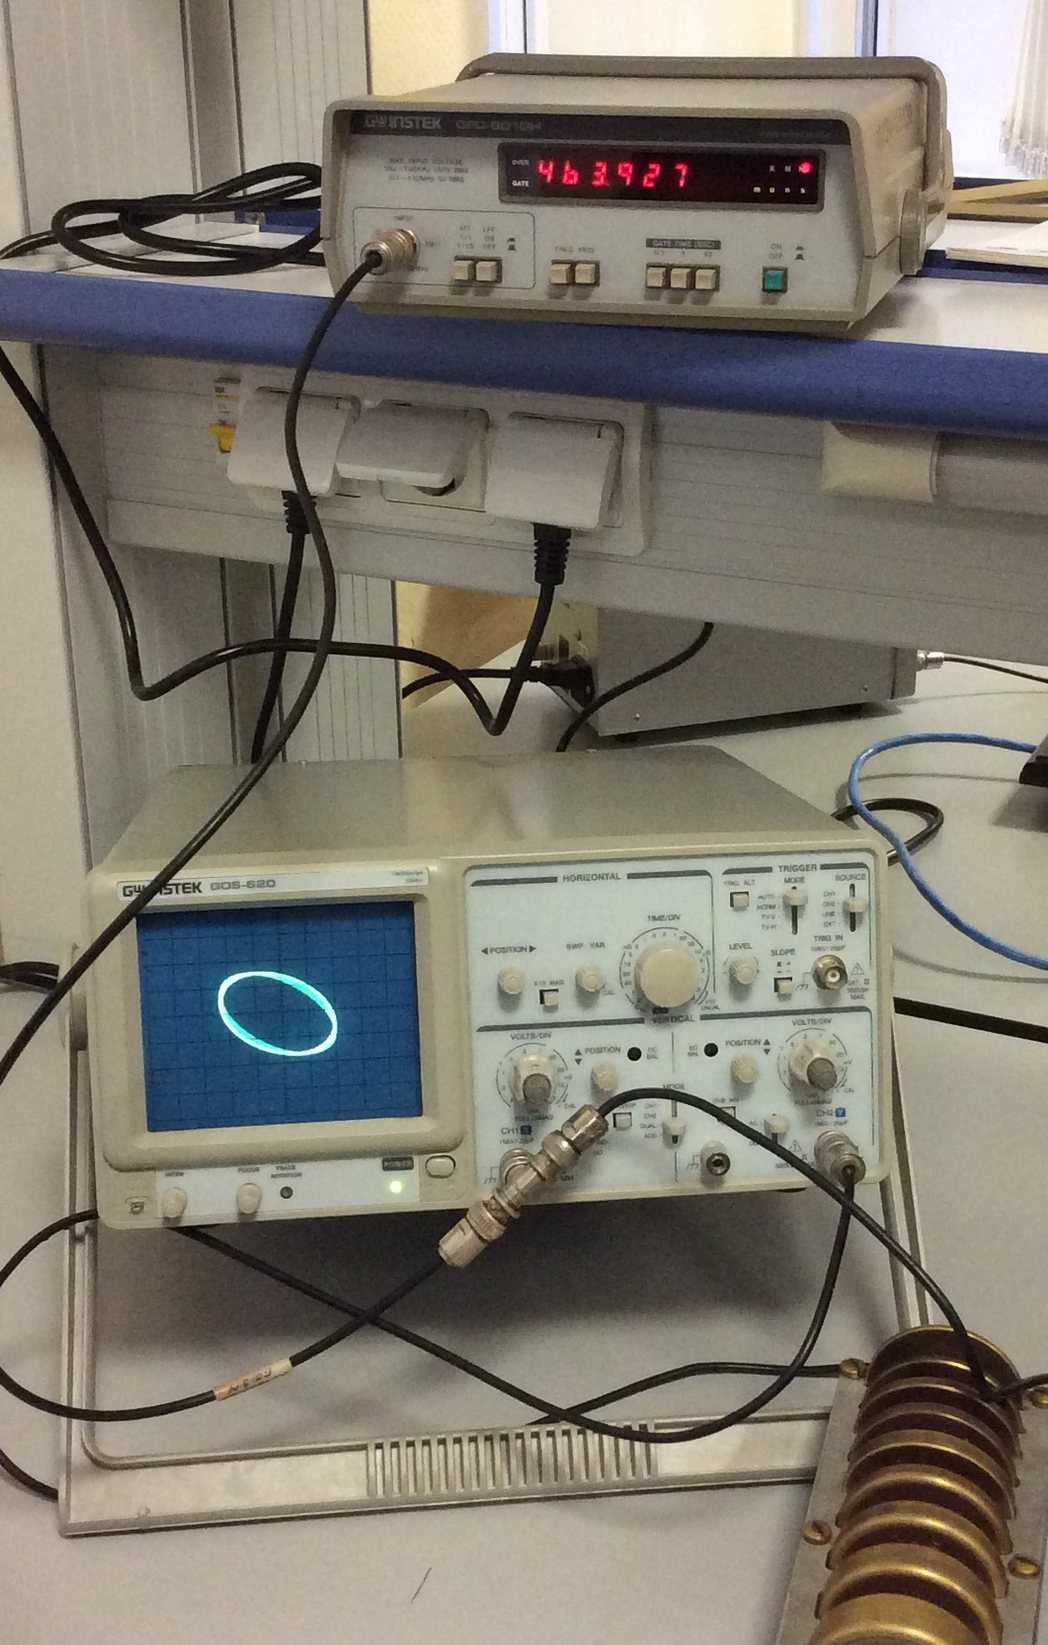
\includegraphics[scale=0.3]{L.png}}
\caption{Фигура Лиссажу, и резонансная частота.}
\end{figure}

\section{Вывод}
Таким образом была исследована вынужденная прецессия гироскопа под действием силы тяжести и сил трения. Была определена скорость вращения ротора гироскопа двумя разными способами, и с учетом погрешности, скорость, определенная через скорость прецессии от силы тяжести, совпадает со скоростью, определенной более точным методам. Исходя из этого можно сделать вывод о том, что соотношение (5) здесь вполне применимо. Так же был оценен момент сил трения, и было показано, что его вклад в прецессию гироскопа мал по сравнению с исследуемым моментом сил тяжести.




\end{document}
